% --------------------------------------------------------------
% This is all preamble stuff that you don't have to worry about.
% Head down to where it says "Start here"
% --------------------------------------------------------------
 
\documentclass[10pt]{article}

 \usepackage{tikz}
\usepackage[margin=1in]{geometry} 
\usepackage{amsmath,amsthm,amssymb}
 
\newcommand{\N}{\mathbb{N}}
\newcommand{\Z}{\mathbb{Z}}
 
\newenvironment{theorem}[2][Theorem]{\begin{trivlist}
\item[\hskip \labelsep {\bfseries #1}\hskip \labelsep {\bfseries #2.}]}{\end{trivlist}}
\newenvironment{lemma}[2][Lemma]{\begin{trivlist}
\item[\hskip \labelsep {\bfseries #1}\hskip \labelsep {\bfseries #2.}]}{\end{trivlist}}
\newenvironment{exercise}[2][Exercise]{\begin{trivlist}
\item[\hskip \labelsep {\bfseries #1}\hskip \labelsep {\bfseries #2.}]}{\end{trivlist}}
\newenvironment{reflection}[2][Reflection]{\begin{trivlist}
\item[\hskip \labelsep {\bfseries #1}\hskip \labelsep {\bfseries #2.}]}{\end{trivlist}}
\newenvironment{proposition}[2][Proposition]{\begin{trivlist}
\item[\hskip \labelsep {\bfseries #1}\hskip \labelsep {\bfseries #2.}]}{\end{trivlist}}
\newenvironment{corollary}[2][Corollary]{\begin{trivlist}
\item[\hskip \labelsep {\bfseries #1}\hskip \labelsep {\bfseries #2.}]}{\end{trivlist}}
\newenvironment{solution}[2][Solution]{\begin{trivlist}
\item[\hskip \labelsep {\bfseries #1}\hskip \labelsep {\bfseries #2.}]}{\end{trivlist}}

\theoremstyle{definition}
\newtheorem*{defn*}{Definition}
\newtheorem{conj}{Conjecture}[section]
\newtheorem{exmp}{Example}[section]
\newtheorem{bas}{Basis}[section]

 
\begin{document}
 
% --------------------------------------------------------------
%                         Start here
% --------------------------------------------------------------
 
%\renewcommand{\qedsymbol}{\filledbox}
 
\title{CS310: Homework 6}%replace X with the appropriate number
\author{Scott Fenton\\ %replace with your name
} %if necessary, replace with your course title
 
\maketitle
\begin{exercise}{(1)}
The following table has the frequencies of symbols in a file, where nl and sp stand for newline
and space, respectively. \\
\\
\begin{tabular}{c|c|c|c|c|c|c|c|c|c|c|c|c|c|c}
Symbols & : & sp & nl  & , & 0 & 1 & 2 & 3 & 4 & 5 & 6 & 7 & 8 & 9\\
\hline
Frequencies & 100 & 605 & 101 & 705 & 431 & 242 & 176 & 59 & 185 & 250 & 174 & 199 & 205 & 217\\

\end{tabular}
\end{exercise}
\begin{exercise}{(1A)} %You can use theorem, proposition, exercise, or reflection here.  Modify x.yz to be whatever number you are proving
Applying Huffman’s algorithm to the data, draw the prefix code tree. The leaves should
be annotated with the symbols and their weights, and internal nodes should be annotated
with the total weights of their substrees. When merging two subtrees, put the lower-weight subtree on the right.
\end{exercise}
 
\begin{solution}{(1A)}
Below is the Huffman Tree\\
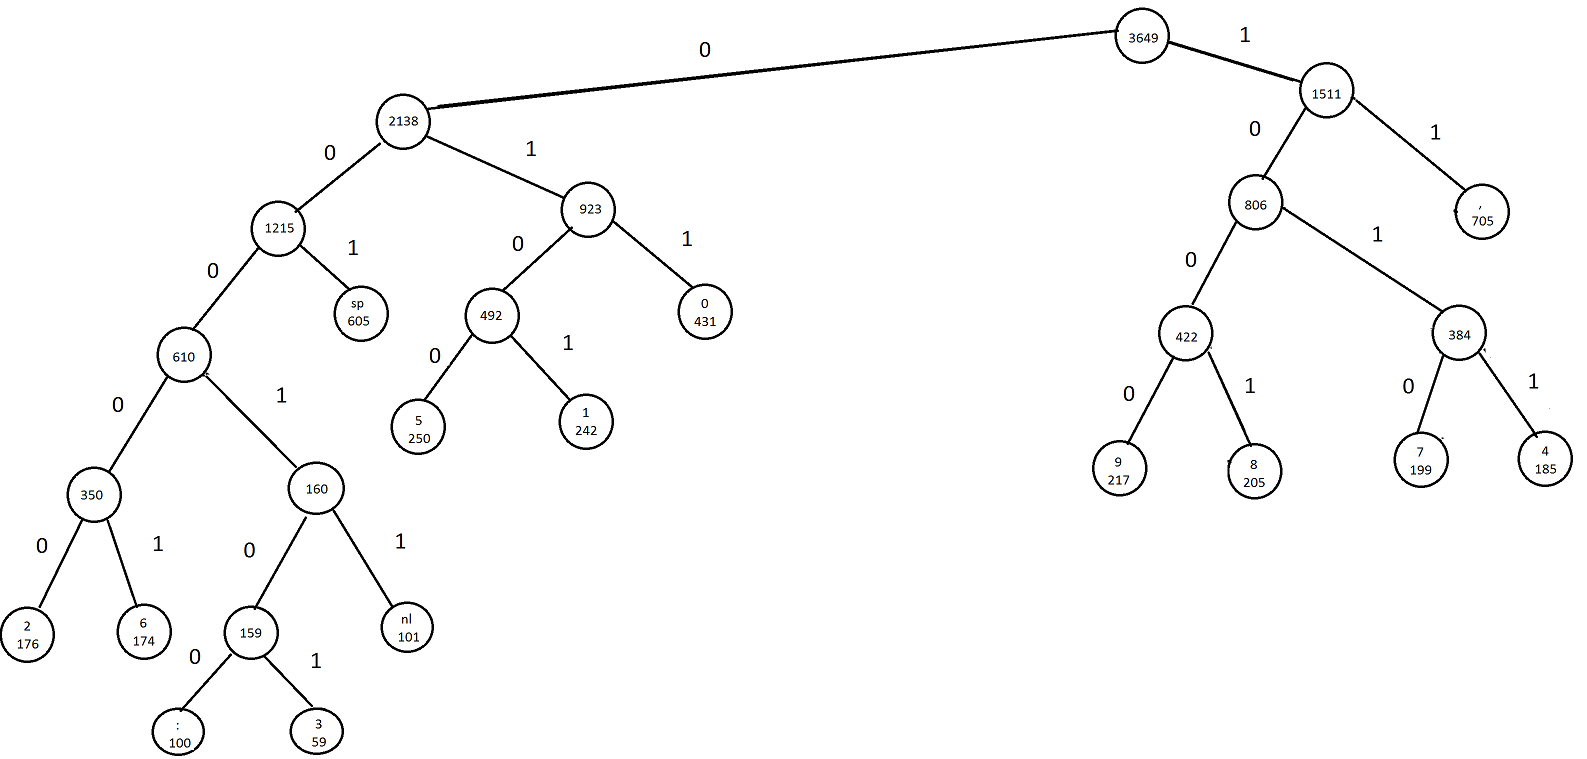
\includegraphics[width=170mm,scale=0.5]{huffman1.PNG}\\
\end{solution}

\begin{exercise}{(1B)} %You can use theorem, proposition, exercise, or reflection here.  Modify x.yz to be whatever number you are proving
Make a table of four columns: symbols, codes, frequencies, total bits, like Slide 20 of
lecture notes.
\end{exercise}

\begin{solution}{(1B)}
Below is the table\\
\\
\begin{tabular}{c|c|c|c}
Char & Frequency & Code & Total bits\\
\hline
, & 705 & 11 & 1410\\
\hline
sp & 605 & 001 & 1815\\
\hline
0 & 431 & 011 & 1293\\
\hline
5 & 250 & 0100 & 1000\\
\hline
1 & 242 & 0101 & 968\\
\hline
9 & 217 & 1000 & 868\\
\hline
8 & 205 & 1001 & 820\\
\hline
7 & 199 & 1010 & 796\\
\hline
4 & 185 & 1011 & 740\\
\hline
2 & 176 & 00000 & 880\\
\hline
6 & 174 & 00001 & 870\\
\hline
nl & 101 & 00011 & 505\\
\hline
: & 100 & 000100 & 600\\
\hline
3 & 59 & 000101 & 354\\
\end{tabular}
\end{solution}

\begin{exercise}{(1C)}
Compress this 7-symbol text: `04: 19,'. Show the result in both binary and hexadecimal.
\end{exercise}

\begin{solution}{(1C)}
The 7-symbol text converted to binary and hex.\\
\\
Binary: 01110110001000010101100011\\
Hexadecimal: 1D88563\\
\end{solution}

\begin{exercise}{(1D)}
Decompress the binary string 11001110111100000.
\end{exercise}

\begin{solution}{(1D)}
The decompressed string is COMMA SPACE COMMA ZERO COMMA TWO.\\
\\
String with quotes: `, ,0,2'\\

\end{solution}

\begin{exercise}{(1E)}
In preparation for fast decoding, sort the codes by lexicographical order like Slide 27 of
lecture notes.
\end{exercise}

\begin{solution}{(1E)}
Char and Code in lexicographical order\\
\\
\begin{tabular}{c|c}
Char & Code\\
\hline
2 & 00000\\
\hline
6 & 00001\\
\hline
: & 000100\\
\hline
3 & 000101\\
\hline
nl & 00011\\
\hline
sp & 001\\
\hline
5 & 0100\\
\hline
1 & 0101\\
\hline
0 & 011\\
\hline
9 & 1000\\
\hline
8 & 1001\\
\hline
7 & 1010\\
\hline
4 & 1011\\
\hline
, & 11\\
\end{tabular}
\end{solution}

\begin{exercise}{(1F)}
Take the top three codes after sorting, and construct the decode array for these three
codes, using . . . to skip repetitive symbols in the decode array, like Slide 28 of lecture
notes.
\end{exercise}

\begin{solution}{(1F)}
Char and bit pattern\\
\\
\begin{tabular}{c|c}
Char & Bit Pattern\\
\hline
2 & 00000000\\
\hline
2 & ...\\
\hline
2 & 00000111\\
\hline
6 & 00001000\\
\hline
6 & ...\\
\hline
6 & 00001111\\
\hline
: & 00010000\\
\hline
: & ...\\
\hline
: & 00010011\\
\end{tabular}
\end{solution}
 
\begin{exercise}{(2A)} %You can use theorem, proposition, exercise, or reflection here.  Modify x.yz to be whatever number you are proving
Apply the Burrows-Wheeler Transform on this string: “abracadabra”, using the methods on
Slides 47 and 48 of lecture notes. Generate all rotations of the string.
\end{exercise}

\begin{solution}{(2A)}
All Rotations\\






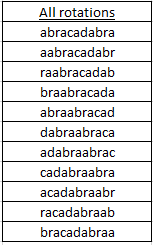
\includegraphics{allrot.PNG}\\
\end{solution}

\begin{exercise}{(2B)}
Reorder the rotations by lexicographical order.
\end{exercise}

\begin{solution}{(2B)}
Lexicographical order\\





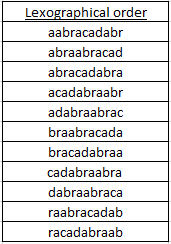
\includegraphics{lexical.PNG}\\
\end{solution}

\begin{exercise}{(2C)}
Output the last column and the index I of the original string. Note that I is zero-based.
See Slide 47.
\end{exercise}

\begin{solution}{(2C)}
The Index I of the original string is 2. \\
\\
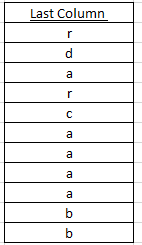
\includegraphics{lastcolumn.PNG}\\
\end{solution}

\begin{exercise}{(2D)}
Write the contents of the three arrays F, L, and T. See Slide 48.
\end{exercise}

\begin{solution}{(2D)}
Contents of FLT:\\
\\
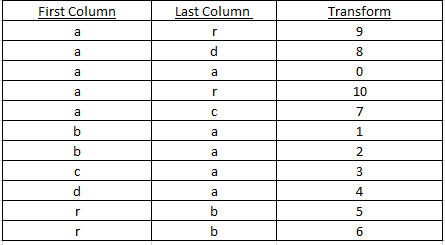
\includegraphics{flt.PNG}\\
\end{solution}


% --------------------------------------------------------------
%     You don't have to mess with anything below this line.
% --------------------------------------------------------------
 
\end{document}